\documentclass[a4paper,twocolumn,12pt]{article}

\usepackage[top=25mm,bottom=25mm,left=25mm,right=25mm]{geometry}

\usepackage{amsmath} 
\usepackage{graphicx}
\usepackage{epstopdf}
\usepackage{url}
\usepackage{setspace} 
\usepackage{float} 
\setstretch{1.44}
\setlength{\columnsep}{6mm}
\usepackage{titlesec}
\titleformat{\section}{\bfseries\large\scshape\filcenter}{\thesection}{1em}{}
\titleformat{\subsection}{\bfseries\normalsize\scshape\filcenter}{\thesubsection}{1em}{}
\titleformat{\subsubsection}{\vspace{-0.7em}\bfseries\small\scshape\filcenter}{\thesubsubsection}{1em}{\vspace{-0.7em}}
\titleformat{\paragraph}{\vspace{-0.7em}\bfseries\small\scshape}{}{1em}{\vspace{-0.7em}}
\setcounter{subsection}{0}

% Following change makes the caption size footnotesize From: http://rorasa.wordpress.com/2010/01/13/instant-latex-command-for-small-figure-and-table-caption/  

\renewcommand{\abstractname}{}    % clear the title
\newcommand{\captionfonts}{\footnotesize}
% \renewcommand\thesection{\Roman{section}.}
% \renewcommand\thesubsection{\Roman{subsection}.}

\makeatletter
\long\def\@makecaption#1#2{
  \vskip\abovecaptionskip
  \sbox\@tempboxa{{\captionfonts #1: #2}}%
  \ifdim \wd\@tempboxa >\hsize
    {\captionfonts #1: #2\par}
  \else
    \hbox to\hsize{\hfil\box\@tempboxa\hfil}%
  \fi
  \vskip\belowcaptionskip}

%\renewcommand\p@subsection{\thesection}
    
\makeatother

\bibliographystyle{h-physrev5}

\begin{document}



%%%%%%%%%%%%%%%%%%%%%%%%%%%%%%%%%%%%%%%%%%%%%%%%%%%%%%%%%%%%%%%%%%%%%%%%%%%%%%%%%%%%
\title{How Metallicity Affects Extrasolar Planets}

\author{George Walker \\
        \small
        Department of Physics, University of Warwick,
        Coventry CV4 7AL, The United Kingdom \\ \small of Great Britain and Northern Ireland}
\date{13/12/23}

\maketitle


%%%%%%%%%%%%%%%%%%%%%%%%%%%%%%%%%%%%%%%%%%%%%%%%%%%%%%%%%%%%%%%%%%%%%%%%%%%%%%%%%%%%

\section{Introduction}
\label{section: Introduction}
\subsection{Objective}
\label{subsection: Objective}
The purpose of this project is to investigate how the metallicity of a star system affects its planets, and to explain this; with a particular focus on sub-Neptunes, which appear to have a trend unlike other types of planets.

%\begin{figure}[h!]
%\centering
%\includegraphics[width=77mm]{DensityMetallicityForDifferentMassRanges.png}
%\vspace{-2mm}
%\caption{The correlation between planet density (indicating planet metallicity, see section \ref{subsection: Basic Assumptions}) and stellar metallicity is positively linearly correlated for most planet mass ranges, but there is a negative correlation for sub-Neptune like planets.}
%\label{fig: DensityMetallicityForDifferentMassRanges}
%\end{figure}

For most mass ranges, the metallicity of the planet is positively correlated to the metallicity of the protoplanetary disk, with the latter being betokened by the system's star, but for sub-Neptunes there is a negative correlation.

\subsection{Importance}
\label{subsection: Importance}
Understanding the relationship between planet properties and system and stellar properties is useful because it allows us to build models which one can either use to predict the properties of planets given the known properties of a star, or compare observations against expectations to infer other parameters influencing the object being observed.

%Investigating the relationship between stellar metallicity and planetary metallicity can provide insight as to the formation of a particular planet.
%-----$>$
Supposing that planet metallicity is influenced by protoplanetary disc metallicity, but also by the formation mechanics of the planet, the models can be used to identify and put constraints on the formation mechanics of the planet by comparing the exoplanet metallicity to the host star metallicity. %Any major discrepancy from the relationship could indicate a wildly different formation.
% - Eh.... I don't think this sounds great

%For example, if the planet metallicity of a rocky body is significantly less than that of a star, and supposing that eccentricity was not something we could calculate, one might be able to say that the planet actually formed outside of the system and was captured by the system it is now in, perhaps after being ejected from an unstable 3-body system.
% - I Like, but this isn't a book so probably not really suitable

%Given that planet metallicity is likely to be indirectly or directly influenced the formation of the planet, comparing the planet against models from the star may also help to identify certain formation mechanics of the planet.

%investigating the relationship between stellar metallicity and planetary metallicity allows us to build models that for any particular planet provides insight as to the formation of the planet.

%Understanding the relationship between planet properties and stellar properties allows us to build models and to predict the properties of exoplanets of given stars. As an example, the metallicity of planets can often affect the atmospheric evolution and also the abundances of molecules needed to sustain life.

Planet metallicity in particular is important because it has been shown to affect the evolution of life, with Shapiro et al. (2023) \cite{Shapiro} recently suggesting that metal rich stars are less suitable for hosting exoplanets with life.

\subsection{Previous Work}
\label{subsection: Previous Work}
%The initial inspiration for this work came from the
It is well established that since a star and its protoplanetary disc form from the same molecular cloud, the composition of a protoplanetary disc should be related to the composition of its star. As dust particles in this disc collide and coalesce, it is expected that planetesimals and then planets which form from the material of this disc will share this composition. Bitsch and Battistini (2020)\cite{Bitsch&BattistiniTheoreticalModel} assume this and then use stellar abundance relationships they derive from 342,682 stars of the GALAH survey to form rigorous models predicting the compositions of solid planetary building blocks and hence Earth-like planetary bodies which form from these, and do this for a wide range of stellar metallicities. Among other relationships, their models predict a positive correlation between stellar metallicity and planetary building block metallicity for blocks exterior to the ice line. This is dominated by a positive correlation between stellar metallicity and iron-mass fraction of the building blocks, but also contributed to by a reduction of the hydrogen mass fraction as stellar metallicity increases.

%https://www.aanda.org/articles/aa/full_html/2023/05/aa43882-22/aa43882-22.html#F2

Adibekyan et al. (2021)\cite{Adibekyan} analyse data from 32 planets and report observing a positive correlation between the iron-mass fraction of a planet and the iron-mass fraction of its star for terrestrial bodies with masses $<$ 10 M$_{\oplus}$. This confirms their initial expectations deriving from the assumption of an abundance correlation between the star and protoplanetary disc, and also agrees with the models of Bitsch and Battistini (2020). They used planetary interior models that they claim are independent of the host star characteristics, depending on the planetary mass, radius, and, Fe/Si and Mg/Si ratios of the host star \cite{SussyInteriorModelsSuper-EarthsAndSub-Neptunes} to estimate iron-mass fractions.

Interestingly however, 
%they also show that planet formation mechanics can affect the relationship, as
5 `super-Mercuries' were identified and followed a different trend, with a positive correlation stronger than when just considering the others. It was supposed that this is because their formation method was different, highlighting the general theoretical importance of formation mechanics on the abundances of material in planetary bodies, and questions the domination of source abundance on the planetary metallicity.
%so that the relationship between planet and stellar abundances is not just dominated by source abundance.

The relationship they find between stellar and planetary iron-mass fractions for the other planets had a correlation with a gradient found to be $4.3\pm0.8$, as opposed to a value of 1 which one might expect, determinedly indicating that planetary formation processes influence the abundances as the planets form from the disc, whilst still suggesting that the original source composition does appear to affect the contemporary planetary abundance of iron.
%Find another\\
%
%There are reports which explain how to use the stellar shit to calculate the planetary parameters (see A$\And$A 633 17 (A10)), but we want to know how do they justify it and how do they empirically back it up. Ok that one specifically tends to just go in for empirical data. Let's see what they have to say anyway. Specially on sub neptunes, but also other types of planets are relevant in my report as well. They just go in for super earths. Fig 11 is a nice one.
%
%Find some for Jupiters.
\\\\Whilst it is well documented that there is an apparent positive correlation between planet metallicity and stellar metallicity for terrestrial, Earth mass planets, curiously, this trend is not seen in all mass ranges. After characterising two sub-Neptunes around a K-dwarf star, Wilson et al. (2022) \cite{Wilson} note that a negative correlation exists between the stellar metallicity and planet density for well-characterised massive ($>$ 10 M$_{\oplus}$) sub-Neptunes, planet density here is assumed to be directly related to planet metallicity. There is as yet no explanation for this trend.

%\subsection{Definitions}
%\label{subsection: Definitions}
%\begin{enumerate}
%    \item A sub-Neptune planet is considered to be Neptune-like planet with less mass than Neptune. In this report, a sub-Neptune planet is any planet with a mass between (10 and 17) earth masses.
%\end{enumerate}

% - Just put this in the neptune theory section

%\subsection{Basic Assumptions}
%\label{subsection: Basic Assumptions}
%\begin{enumerate}
%    \item A star's metallicity is shared by the protoplanetary disk it formed from (citation needed - see one of the papers I read), and hence the star is an indication of the disk that a planet formed from. Planets form from material in the protoplanetary disk.
%    \item The density of a planet can indicate its metallicity
%\end{enumerate}
% - Kind of a weird section now that I'm going to rigourously go through this in the theory section. The placement was deliberate to sort of explain the purpose etc nicely but I think I'm just going to stick all the theory in the theory and people can work it out from there. I'll probably reference some assumptions in the intro section but just expect them to be explained by the theory section.

\subsection{Approach - Planet-Stellar Metallicity relationship}
\label{subsection: Approach}
%The factors affecting the metallicity of the planet need to be identified, and generally(by this I mean: as an intuitive conclusion) that's the source abundance of metal and then the formation and evolution mechanics of the planet.

The factors affecting the metallicity (the ratio of iron to hydrogen) of a planet need to be identified, and generally there are three factors affecting this: The source abundance of metal and hydrogen, the formation mechanics of the planet from this material and the evolution mechanics of the planet. An understanding of all three is required to fully understand the situation.

The reliability of any data providing information into these may also affect the reliability of conclusions or inferences made.


%Within the source aboundance of metal, the source is the p.p disk
\subsubsection{Source Abundance}
The source of the iron and hydrogen is the protoplanetary disk from which the planets form. %(Trust me bro).
The protoplanetary disc and the star are thought to have originally formed from material in the same molecular cloud and thus the stellar metallicity, which can be calculated directly from observations, is generally assumed to be a reliable indication of the protoplanetary disc composition. This will also be assumed here.

%A correlation between the stellar metallicity and the abundance of metal in the protoplanetary disc is assumed since both are thought to have originally formed from material in the same molecular cloud, and thus the stellar metallicity, which can be calculated directly from observations, is an indication of the protoplanetary disk.

%(again, trust me bro). I mean, could actually test this by finding some binaries or something lol.

\subsubsection{Formation Mechanics and Evolution}
Within the formation and evolution mechanics there are potentially a number of dynamics of the formation methods which would lead to relations between disc metallicity and planet metallicity. An understanding of the formation mechanics is needed to describe the time evolution of Fe and H abundances and identify any particular reasons for a given trend. The significance of formation has already been shown empirically by Adibekyan et al. (2021).
% identify any particular reasons = explain and describe the processes

%The final thing in the chain to to analyse is the certainty of the metallicity measurements since these are currently just inferred by the planet density. It is possible that these models are flawed.

%(by this I mean: there could be multiple dynamics affecting it, or maybe 0. Intuitively the dynamics of formation would affect the gathering of metal for the resulting planet. Some of these are known, but no certainty that all of the dynamics are known)

\subsubsection{Measurements and Their Uncertainties}
The end nodes in the chain to analyse are the certainty of the metallicity measurements. The stellar metallicity measurements are assumed to be accurate since the metallicity values are inferred from spectroscopy. There is some uncertainty in the assumption of a relationship between stellar and disc composition, but it will be assumed here that one may still expect them to be statistically related, which would reveal itself when considering many data. The planet metallicity values may have more uncertainty since these are currently only inferred via models involving planet density and some constraints provided by the star. There is much degeneracy involved in these models, as discussed in section \ref{subsection: Planet Metallicity Models}, and any models which use stellar parameters will introduce intrinsic relationships between the planet metallicity and stellar metallicity, so care must be taken when analysing and explaining this relationship.

%And why cant we use spectroscopy - the areosols, but that goes in the theory right?

%To the point below: I think I may have sort of oversimplified it a bit and in fact there are sort of more rigourous approaches. Density does tend to be assumed to be related to metallicity a lot and they do tend to just ignore plotting metallicity for a lot of planets which is a problem, and one which I do actually want to address in this approach section because I beleive planet density is too far removed from metallicity to be used in relationships, especially when clearly the field has some quite complex mechanics which appear to go against what feels intuitive.

However, when presenting trends, the planet density is often used as a substitute for planet metallicity \cite{Wilson}, with the two being assumed to have a linear relationship. This should not be done without justification. It is possible that these density-metallicity models are flawed. As such, the approaches taken here will be to justify that relationship with a more rigorous model when planet metallicity values are not available, and where metallicity values have been derived through more complex models, use planet metallicity as one of the components in any relationship that is being attempted to be displayed, however uncertain these values may be. Where planet metallicity values are not available, this work may make use of models to predict these. This reduces the amount of assumptions made.

%Using metallicity as one of the components in any relationship that is being attempted to be displayed (however uncertain this may be) is a more rigorous approach than using the density and assuming positive linearity when drawing conclusions.

% They're completely flawed because we use density and don't even bother finding the density-metallicity relationship, and I've shown it to not be linear. We need to be plotting metallicity not density ffs.

%I wonder whether the sub-Neptunes retain their alpha/Fe metallicities.

%%%%%%%%%%%%%%%%%%%%%%%%%%%%%%%%%%%%%%%%%%%%%%%%%%%%%%%%%%%%%%%%%%%%%%%%%%%%%%%%%%%%

\section{Theory}
\label{section: Theory}

%There could be instances that require you to have multiple equations:
%
%\begin{eqnarray}
%x_1 &=& A y_1 + B y_2 + C y_3    \,, \\
%x_2 &=& D y_1 + E y_2 + G y_3    \,, \\ 
%x_2 &=& H y_1 + I y_2 + J y_3    \nonumber\\
%    &~& + K y_4 + L y_5 + M y_6  \,. 
%\label{eq: eq_2}
%\end{eqnarray}
%
%
%\begin{figure}[t!]
%\centering
%\includegraphics[width=77mm]{pngexample.png}
%\vspace{-2mm}
%\caption{}
%\label{fig: fig_1}
%\end{figure}

\subsection{System formation}
\label{subsection: System formation}
The protoplanetary disc and the star are generally thought to both be made up of material that originated from the same molecular cloud, and as such, the composition of star and disc should be similar.% [Could do with a reference]

%All forms from same cloud so yeah it follows that it should be similar. Essentially the supposition is that the stellar composition should be a direct indication of the protoplanetary disk composition and hence the stellar composition can be used as the protoplanetary disk composition. Stellar metallicity doesn't directly affect the exoplanet metallicity but the stellar metallicity indicates the protoplanetary disk metallicity which is considered to have an affect on the planets.

%In the planetary disk accretion model, the 

\subsection{Types of planets and their formation methods}
\label{section: Planet formation}
\subsubsection{Terrestrial}
Terrestrial planets are defined here as being rich in rock and ice but without a large gaseous envelope. Terrestrial planets with masses greater than 1 M$ _\oplus$ may be referred to as `super-Earths'.

Their formation is not greatly understood, and the field is too rich to do it justice here \cite{EarthFormation}. As a general overview, terrestrial planets are thought to begin as dust 'clumps' together to form planetesimals.  The process for this clumping is greatly debated. At the mass scales of planetesimals, gravitational forces begin to dominate and collisions occur, forming planet embryos. Planet embryos can eventually form into terrestrial planets if they can form a stable orbit without being ejected or perturbed by more massive planets. A second proposed method is the formation of planetesimals from pebble accretion \cite{PebbleAccretion}. A more detailed review of terrestrial planet formation was written by Morbidelli et al. (2012) \cite{EarthFormation}. 

%\subsubsection{Neptune (Ice Giant)}
\subsubsection{Sub-Neptune}
There is currently no clear definition for what a sub-Neptune is. Here, we define a sub-Neptune as any planet with a mass less than that of Neptune but with the distinctive features of Neptune, that is, having a solid core of rock and ice, with a large hydrogen and helium envelope. A rocky planet without a large hydrogen and helium envelope may be referred to as a `super-Earth', although the dividing line is not clear.

Sub-Neptunes are not well understood as observations on exoplanets has only recently been made possible and there are no analogous planets within the solar system.

%\cite{https://doi.org/10.3847/1538-4357 2Fab6ffb}

Bean et al. (2021)\cite{NatureAndOriginOfSubNeptunesGoodPaper} analyse the formation of sub-Neptunes and describe two plausible formation pathways. The first method, the `drift model' involves pebbles which drift inwards until they reach equilibrium points referred to as `pressure bumps'. From there, it is supposed that they grow through accretion and collisions to form planetary embryos and eventually planets. As pebbles formed outside of the ice line drift inwards, their volatiles are lost, and pebbles formed within the ice line will have less volatiles to begin with, so the planetary embryos which form out of these should have a low abundance of volatiles.

The `migration' model supposes that large cores form in all parts of the disc through accretion. This process occurs at a quicker rate outside of the ice line. The cores then migrate inwards, after which they collide with each other to grow. In this model the cores are able to retain more of their volatiles.

In both scenarios, the cores then accrete gas from the disc, forming gaseous envelopes around them. After formation, the bodies bifurcated into two distinct classes of planet based on their ability to retain a hydrogen atmosphere. Bodies above a certain radius are able to retain their atmospheres and we may call these `sub-Neptunes', whilst bodies below a certain radius have their atmospheres stripped, becoming what one may refer to as `super-Earths'. Atmospheric loss mechanisms are not fully understood.

%\subsubsection{Gas Giant}
% If I get time this may be quite useful, especially since it addsa another size range and all together ot adds to the total understanding and processes

\subsection{Planet metallicity models}
\label{subsection: Planet Metallicity Models}
\vspace{-0.3em}
Spectroscopy on planets themselves is hard to achieve with current equipment, and so deriving the metallicity of a planet must be done through compositional models of interior structure. There are a wide variety of models used to do this, including those by Dorn et al. (2017) \cite{SussyInteriorModelsSuper-EarthsAndSub-Neptunes} and the methods employed by Mortier et al. (2020) \cite{MortierInteriorStructure}. Models of interior structure suffer from much degeneracy, since the only data available are the bulk density of the planet and some stellar parameters. As discussed earlier, any models which involve stellar parameters will introduce intrinsic relationships between planet and stellar metallicites which may not really exist.

\subsection{Planet density - planet metallicity relationship}
%Someone et al used 6 sub neptune planets characterised with spectroscopy to build a model for how the metallic metallicity and composition can be modelled using the density and some other shit. These models are reasonably certain.
%See how Wilson did it.
%See 5.1 and 6.2. 5.1 is the main start of it. "Bayesian"
%7 of leleu et al - 7.4 looks more specific. "Bayesian analysis"
%Also 7.1 says something about metals which is the main focus. Does it relate to density though, possibly not.
%Might still be useful as a section here though.
%Well it looks like it uses the star anyway to work out the planet stuff so one can't then just compare the metallicity to star metallicity. Ofc it will be correlated because u worked it out from that.

%There's basically nothing on this. This is stupid. No wonder why it's negative because there's basically no theory on it whatsoever.

%Well it sort of looks like they sort of use the radius and mass and take the stellar parameters as well to model the interior structure of the planet.

%Eh, can we really rigorously assume that the planet metallicity is related to its density? Eh, yes kind of if we looked at the composition of such planets. Methods of internal structure analysis allude to the idea of the metals making up the density bits. I mean sure yeah metals are more dense. We can probably just propound that intuitively.
%I haven't found a rigorous way of doing it though, but oh well.
%If we had a DB of actual metallicities which are calculable then we could do the relationship empirically, and also just use the metallicities in the planet-stellar metallicity relationship instead, although we don't get as much data by doing that.


%The real issue though is that the metallicity itself is kind of modelled based on the stellar metallicity and that's not really the idea...

%Density therefore provides a cleaner, more direct method.

%Coming at metallicity through density through an intuition notion removes the issue of the metallicity being based on stellar metallicity just because of the way it was calculated.

%So:
Since planet metallicity values are not simple to calculate, and are often calculated from stellar composition parameters, it cannot always be reliably used when attempting to find a relationship between planet and stellar metallicity. Instead, it is often assumed that the density of a planet is correlated to its metallicity, and therefore that density, which can be measured with great precision, can act as a substitute for planet metallicity when exploring trends. By assuming the mass and thus density is only contributed to by the iron and hydrogen the density is related to the metallicity as,
\begin{equation}
\rho = \frac{1 + 1226\times10^{[Fe/H]}}{\frac{1}{0.09}+\frac{1226\times10^{[Fe/H]}}{7.874}}
\label{equation1}
\end{equation}

It is also assumed that the densities of H and Fe are constant with radii. The assumptions made here are not necessarily appropriate ones to make, but the model highlights the non-linear relationship between planet density and planet metallicity and where planet metallicity values are not available, a model such as this may be used, although this should only be done in appropriate circumstances.

%but I spent so long on this that I think I'd rather spend a bit more time justifying that than throwing out my model. If nothing else then it's at least an improvement. I recon more materials should be included in the model but that's harder to do, also going to need a lot of paper or wolfram alpha. Also though, it's not possible to try to calculate all of the planet composition values without using some of the stellar properties so Fe/H from density will have to do.
%. A simple hydrostatic equilibrium model would do it right?

%Is wrong anyway because I use e and not 10

%Ok. Fine. That works. That's a relief. Phew. That's that section of the theory done and justified. Will need polishing but at least we know we have it justified now, and got to stick in a formular.

% Could add the graph in. Could add a graph with multiple lines in showing the uncertainties in the model.

% Here, consider the other things affecting density as well though, especially opposing the trend. Water for example. When Fe/H goes up, exterior to the water-ice line, oxygen goes down, but not as much as H (although really we need to know H2), which means less water and thus more H and thus lower density. This affect may be really small and negligible though but we can't just discard shit like that without actually quanitfying its affects first. Well, seems like most of the oxygen gets put in CO2 anyway or something. I suspect though that hydrogen still dominates the mass. Ok it looks like from fig 10 that as metallicity increases, the water content shoots down anyway because the silicates increase in abundance. Water not shown on interior plot again.

%This relationship  is beautifully confirmed by the idiots over at the science journal paper who literally instead of plotting an exponential plot two straight lines at different points in the data, say it's linear and call it a day.

\subsection{Metallicities within the Milky Way}
\label{subsection: Metallicities within the Milky Way}
The average metallicities of stars in the Milky Way vary depending on their location. The metallicities of stars in the thick disk are typically less than that of the Sun \cite{ThickDisc}, whilst in the thin disk the metallicities are higher \cite{ThinAndThickDiskKinematics}.

Kilic et al. (2017) \cite{MilkyWayMetallicitiesNearbyWDs} use nearby white dwarfs to estimate the age of stars in the different parts of the galaxy, and this is shown in figure 1.
\begin{figure}[h!]
\centering
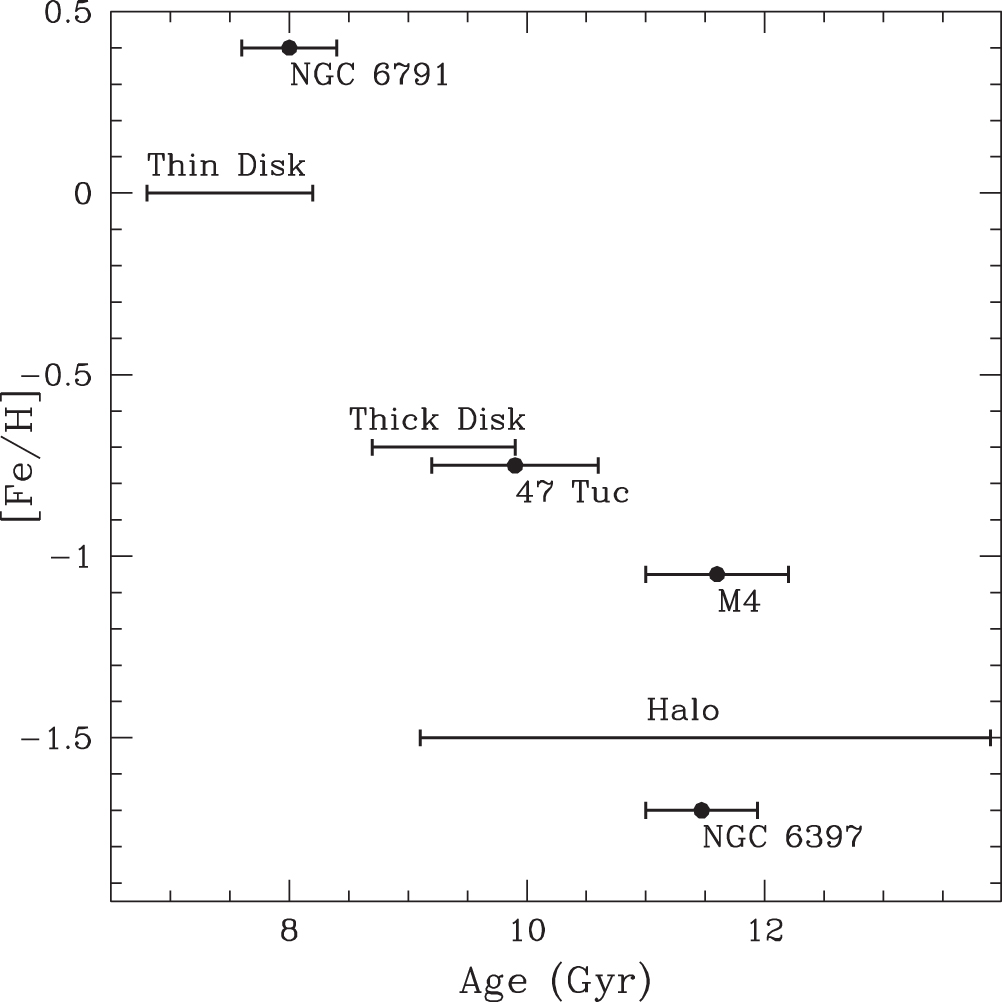
\includegraphics[width=77mm]{apjaa62a5f10_hr.jpg}
\vspace{-2mm}
\caption{The estimated age and metallicities of white dwarfs in different parts of the galaxy. This figure was produced by Kilic et al. \cite{MilkyWayMetallicitiesNearbyWDs}.}
\label{fig: Age-metallicity for WDs}
\end{figure}

The location of a star in the Milky Way can be estimated using its galactic velocity. Vieira et al. (2022)\cite{ThinAndThickDiskKinematics} used data collected by ESA's GAIA to show that the average values of components of the galactic velocity of stars differs depending on whether they are in the thick disk or thin disk. This was also demonstrated by \cite{ThickDisc}.

Finally, there exists a negative correlation between alpha/Fe and Fe/H metallicities throughout the galaxy, as shown by Afşar et al,. (2012) \cite{Afşar}.

%\subsection{Hydrostatic equilibrium effects}
%Start taking affect above 50Me so makes no difference for us.


%\subsection{Observational Biases}
%\label{subsection: Observational Biases}

\section{Methodologies}
\subsection{Data}
I retrieved data on exoplanets from the NASA Exoplanet Archive \cite{NASA Exoplanet Archive}, and used the coordinates of their star, along with its GAIA magnitude as declared in the NASA data to retrieve further data on the star from the ESA GAIA archive \cite{GAIA Archive}.

\subsection{Analyses}
Statistical analyses were done using an mmmc analsyses, using code originally wrote by some italian dude and then modified by tom



%%%%%%%%%%%%%%%%%%%%%%%%%%%%%%%%%%%%%%%%%%%%%%%%%%%%%%%%%%%%%%%%%%%%%%%%%%%%%%%%%%%%
\section{Results}
The empirical affect of metal on a planet is different depending on what `type' of planet it is, as defined in section \ref{section: Planet formation}.
\subsection{Affect of Stellar Metallicity, [Fe/H]}

\subsubsection{On Radius of Planet}
\begin{figure}
    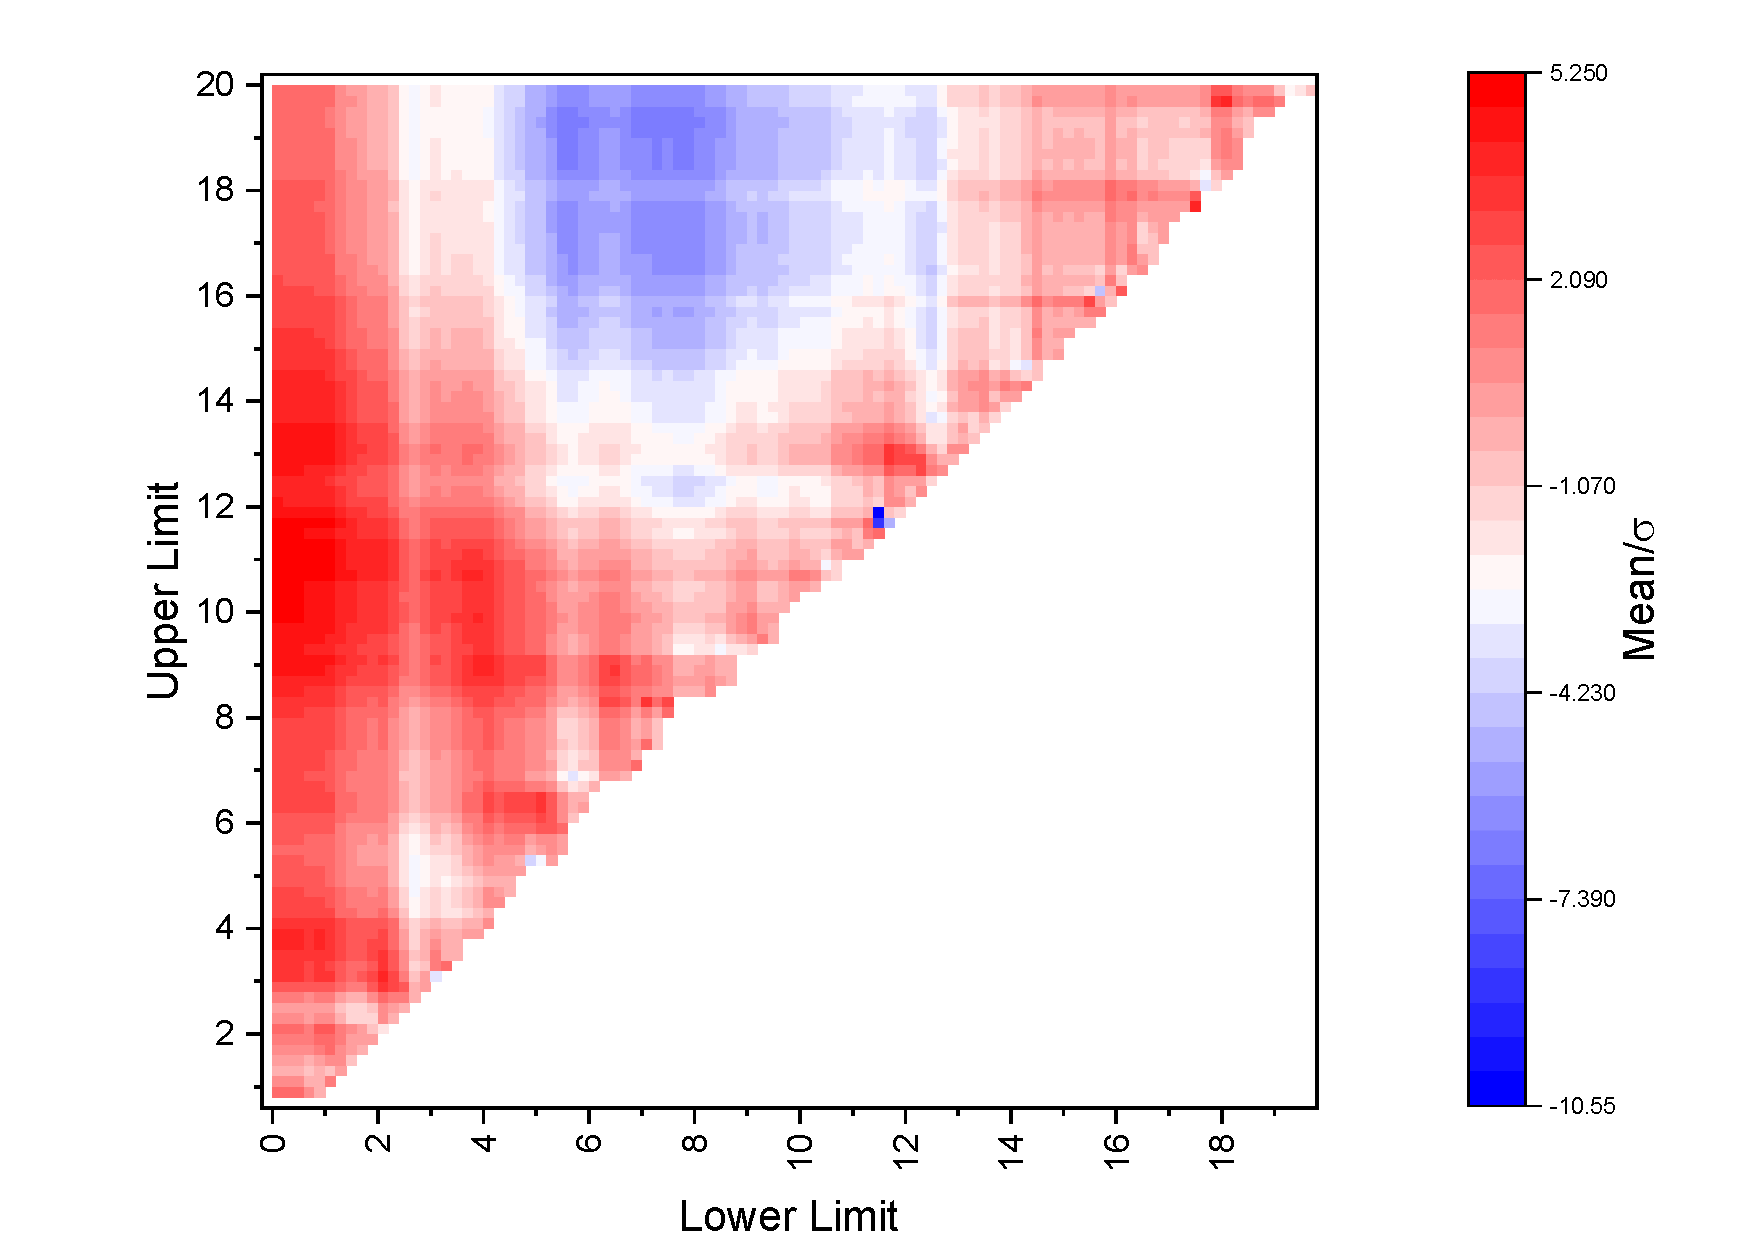
\includegraphics{FeH vs radius correlations.pdf}
    \caption{P-value of the correlation between planet radius and host start metallicity normalised by the standard deviation of that correlation, presented for values across a continuum of different radii ranges.}
    \label{fig:enter-label}
\end{figure}

Data on planets below a radius of 1.6 were statistically insignificant, and the rate of change of correlations was not smooth when adjusting the range.


\paragraph{Radii below 1.6 Earth radii}


\subsection{Metallicity of exoplanets}



%%%%%%%%%%%%%%%%%%%%%%%%%%%%%%%%%%%%%%%%%%%%%%%%%%%%%%%%%%%%%%%%%%%%%%%%%%%%%%%%%%%%


%\setlength{\itemsep}{-2mm}
\vspace{-1em}
\footnotesize\bibliography{LaTex_References}

%\end{thebibliography}
\end{document}
